\documentclass[CS4204-Notes.tex]{subfiles}
\begin{document}

\section{Parallelism basics}
\subsection{Definitions}
\begin{figure}[H]
\centering
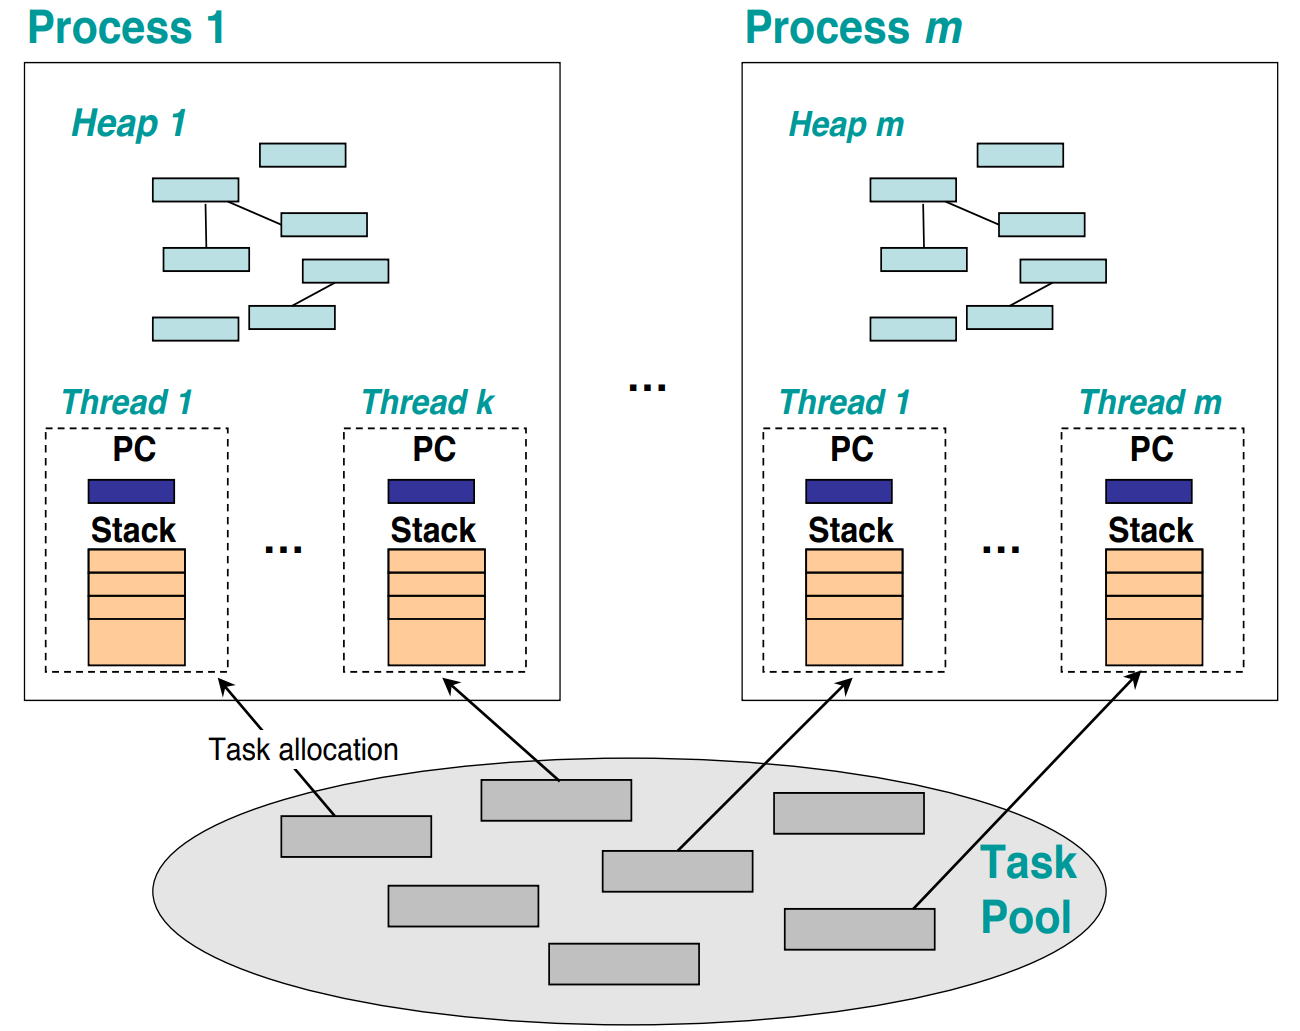
\includegraphics[width=0.6\textwidth, keepaspectratio]{imgs/terminology.png}
\caption{Diagram of how parallel processes are split up into threads and tasks.}
\end{figure}
\noindent
\textbf{Process} - A process is an independent unit of computation with private address space and usually comprises of multiple threads. The process-thread model does not include registers so it is not hardware-specific. 
\n
\textbf{Task} - Indicates a unit of computation that has been identified by the programmer, for example in a workpool setting and is often used synonymously with thread.
\n
\textbf{Thread} - The basic unit of parallel computation. It is lightweight and shares address space with other threads in the same process, but has its own separate stack and program counter. 
\n
\textbf{Filament} - Filaments wind together to form threads. These are primitive units of pure computation which does no communication. Filaments don't necessarily need context switching if they are small enough because they will terminate with a result. 

\subsection{Granularity}
Granularity is a \textbf{relative} measure of the ratio of the amount of computation to the amount of communication within a parallel algorithm implementation. In other words, it is a term used for the size of a parallel task in terms of its execution time. 
\n
For example, \textbf{coarse-grained} tasks are larger and relatively few in number while \textbf{fine-grained} tasks are smaller but in larger numbers. If a program is too coarse-grained, then there is not enough parallelism, resulting in poor utilisation. On the other hand if a program is too fine-grained, the overhead of thread creation and communication overtakes the benefit gained from parallel computation. A big issue in parallelism is determining the optimal granularity of a task.
\begin{figure}[H]
\centering
\begin{subfigure}{0.47\textwidth}
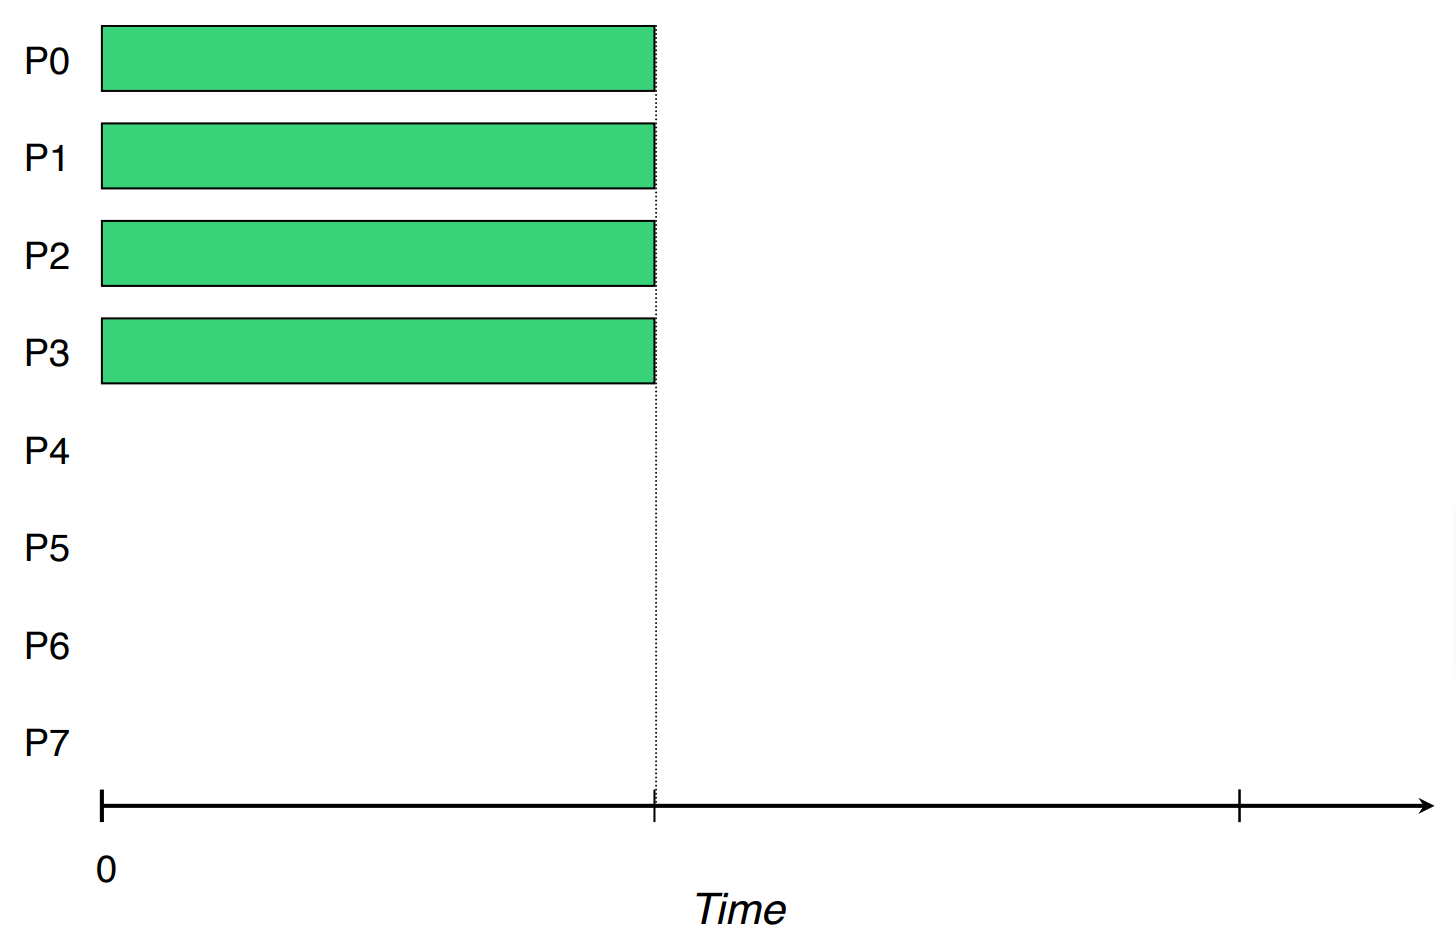
\includegraphics[width=1\textwidth, keepaspectratio]{imgs/granularity-little.png}
\caption{Too little granularity}
\end{subfigure}
\hspace*{\fill}
\begin{subfigure}{0.47\textwidth}
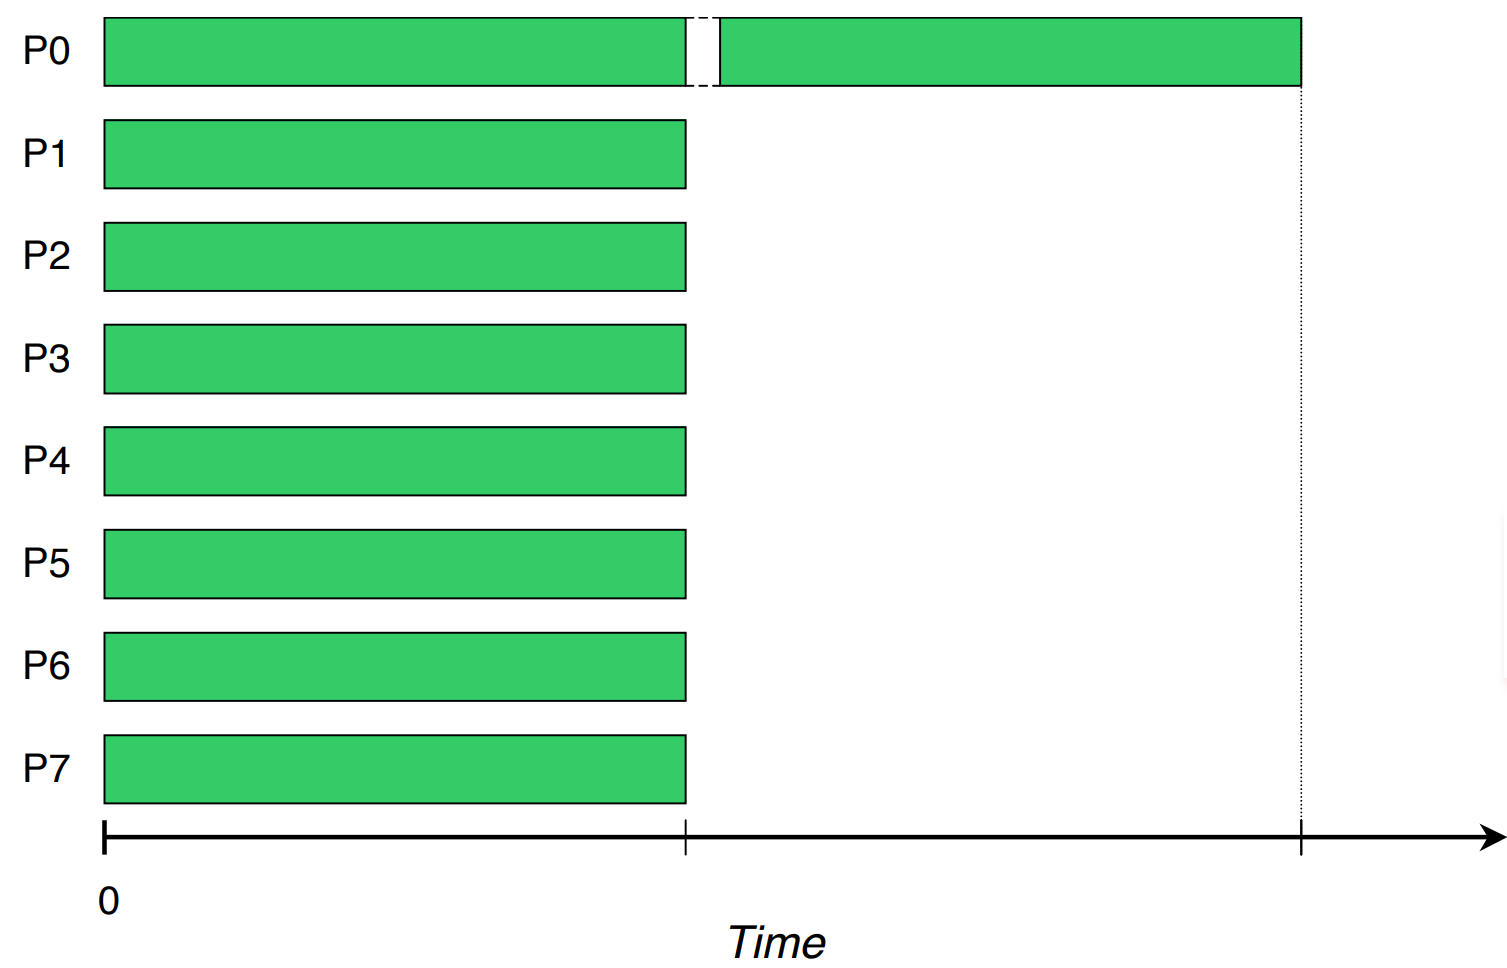
\includegraphics[width=1\textwidth, keepaspectratio]{imgs/granularity-much.png}
\caption{Too much granularity}
\end{subfigure}
\end{figure}
\noindent
The granularity is partially determined by three characteristics of the algorithm to parallelise and the hardware used to run the algorithm.
\begin{itemize}
\item \textbf{Structure of the problem} - Algorithms that are inherently \textit{data-parallel}, that is few unique operations are done over many pieces of data are often fine-grained by definition, as the same operation is applied to all the data. On the other hand, if only larger subroutines can be executed in parallel which require many calculations and little communication, then they are inherently coarse-grained. 
\item \textbf{Size of the problem} - Given 10 data elements and 10 processing elements (PEs), then only 1 clock cycle is required to process all 10 elements in parallel. However if the problem size is increased to 100 elements, then each PE now has to work on 10 elements each. This implies that larger sized tasks are more coarse-grained by default.
\item \textbf{Number of processors} - By the same token as the size of the problem, the number of processors also directly affects granularity as there are only so many limited processing units. More processors would lead to more fine-grained granularity as each processor has to do less, provided the size of the problem stayed constant. 
\end{itemize}
Granularity is important in choosing the most efficient paradigm of parallel hardware for the algorithm at hand. For example SIMD architectures are best for fine-grained algorithms while MIMD architectures are less effective due to the message-passing needed between MIMD cores. This further indicates that communication speed is a factor in choosing granularity, as a fine-grained task would be heavily hampered by slow communication while coarse-grained tasks would be effected less. 

\subsection{Amdahl's law}
Amdahl's law is a law which governs the speed-up of parallelism on a given problem. It is used as a way to determine limits on parallel optimisation. It states that if the proportion of sequential work performed by a program is $s$, then the maximum speedup that can be achieved is $\frac{1}{s}$. This may be expressed in the equation:
\begin{equation}
\text{Speedup} = \frac{1}{s + \frac{p}{N}}
\end{equation}
where $N$ is the number of processors available and $p$ is the amount of time spent on parallel parts of the program that can be done in parallel. 
\begin{figure}[H]
\centering
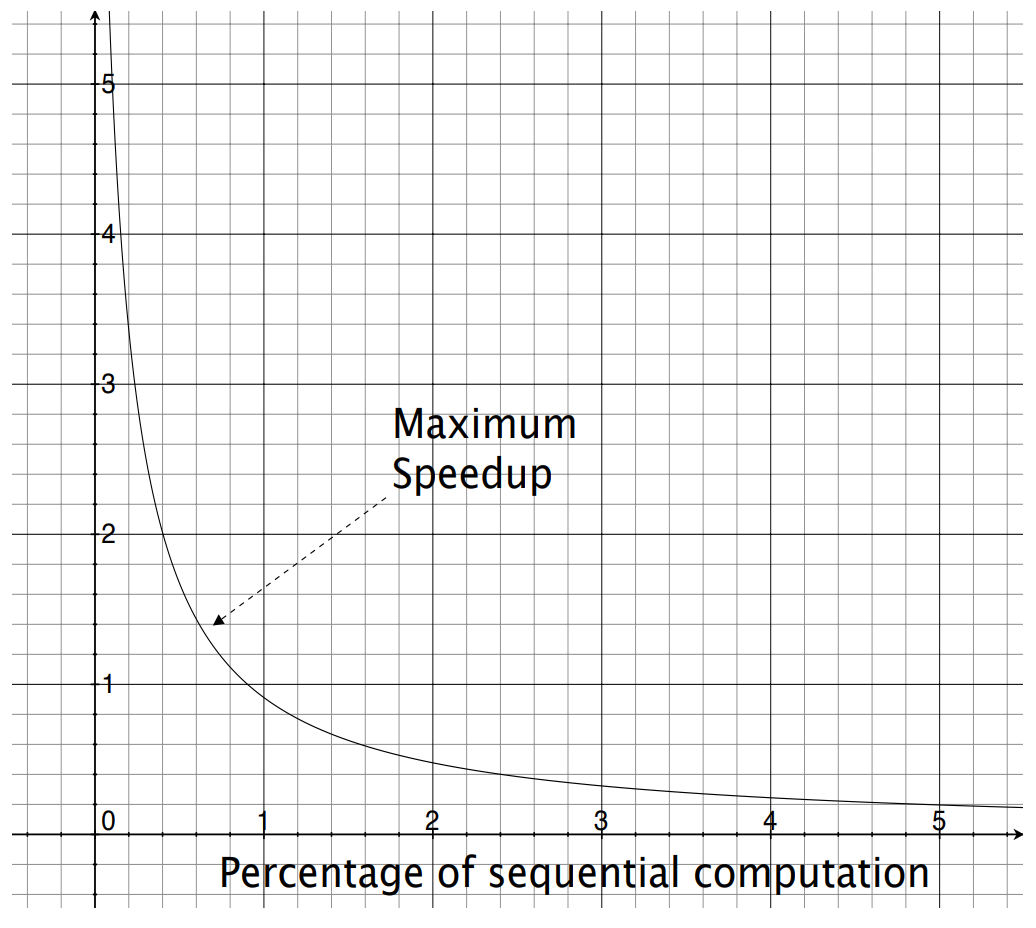
\includegraphics[width=0.5\textwidth, keepaspectratio]{imgs/amdahls-law.png}
\caption{The effect of Amdahl's law on parallel computation. The $y$-axis shows the maximum speedup that can be achieved if the problem size remains fixed.}
\label{fig:amdals-law}
\end{figure}
\noindent
The graph in figure \ref{fig:amdals-law} shows that to achieve a high speedup, only a tiny percentage of the total execution time can be sequential. This means the need for sequential operations heavily dominates computation time, and a lot of parallelism is needed to get any good speedup. 
\section{Parallel Haskell}
Writing explicit parallel programs is very difficult as there are many things that have to be specified by the programmer, most notably:
\begin{itemize}
\item Task identification
\item Task Creation
\item Task placement
\item Data placement
\item Load balancing
\item Communication
\end{itemize}
Having to deal with all this at a low-level of program is prone to errors, which is why additional abstractions are required. \textbf{Glasgow Parallel Haskell (GpH)} aims to solve this by using an approach where the runtime system manages parallelism which is introduced by the parallel programmer. The goal is to create a simple parallel language extension and \textit{automatic} control of parallelism. GpH procides a simple basic model for parallelism, programmable for both task and data parallelism. It communicates through a virtual shared heap and is architecture independent. 
\n
A purely functional language like Haskell has several advantages when it comes to parallel execution.
\begin{itemize}
\item No side effects - because there are no side effects, it is always safe to execute computations in parallel and the results will be the same regardless of the order. More strongly, the result will be identical to running the program sequentially.
\item No race conditions - because the order of I/O operations is fully defined by the language, no race conditions or unexpected outputs can occur from interleaving I/O operations in the wrong order.
\item No deadlocks - data and control dependencies in the functional language ensures that there can be no unresolved mutual dependencies between tasks.
\end{itemize}

\subsection{The \texttt{par} and \texttt{pseq} annotation}
The primitive, higher-order function \texttt{par} is used by the programmer to mark a sub-expression as being suitable for parallel evaluation. It is the basic way to introduce parallelism in GpH.
\begin{lstlisting}[caption={Example of the \texttt{par} annotation.}]
-- Create a spark for a and return the value of b
a `par` b

-- Spark x and return f x
x `par` f x where x = ...
\end{lstlisting}
\begin{lstlisting}[caption={Example of the \texttt{pseq} annotation.}]
-- Evaluate a and return the value of b
a `pseq` b

-- First evaluate x, then return f x
x `pseq` f x where x = ...
\end{lstlisting}
The \texttt{par} annotation is an example of the programmer exposing parallelism to the compiler without explicitly forking threads with concurrent methods. The expression \texttt{a `par` b} \textit{sparks} the evaluation of \texttt{x} and returns \texttt{y}. Sparks are queued for execution in FIFO order, but are not executed immediately. The runtime system determines if the spark is converted into a real thread when it detects an idle CPU. This way the parallelism is spread among real CPUs but it is not a mandatory scheme. 
\n
While \texttt{par} creates new sparks, \texttt{pseq} and \texttt{seq} ensures sequential evaluation. The two are almost equivalent, the difference being that \texttt{seq} can evaluate its arguments in either order, but \texttt{pseq} must evaluate the first argument before the second, allowing the programmer to control evaluation order in conjunction with sparking with \texttt{par}.
\lstset{escapeinside={<@}{@>}}
\def\textquoteback{\`{}}
\begin{lstlisting}[caption={Parallel Fibonacci}]
import Control.Parallel

pfib :: Int -> Int
pfib n 
	| n <= 1 = 1
	| otherwise	= n2 <@\textcolor{red}{\textquoteback par\textquoteback}@> (n1 <@\texttt{\textcolor{red}{\textquoteback pseq\textquoteback}}@> n1 + n2 + 1)
		where
			n1 = pfib (n-1)
			n2 = pfib (n-2)
\end{lstlisting}
\texttt{par} is used to spark a thread to evaluate \texttt{n1} and \texttt{pseq} is used to foce the parent thread to evaluate \texttt{n2} before adding the two sub-expressions back together. When using \texttt{par}, the general rule of thumb is that the sparked computation should be required at a later time, but not too soon. The sparked computation should not be too small, otherwise the cost of forking it in parallel will be too large relative to the amount of parallelism gained. The runtime system decides on issues such as when and where threads are created and the communication between threads. Most notably, it determined whether a thread is created or not. This parallelism model is therefore called \textbf{semi-explicit} as the programmer only marks which areas can be parallelised, and the runtime system decides whether to execute the sparks in parallel based on information during execution such as the system load and processors available. This approach eliminates the complications of low-level parallelism, leaving responsibility of these issues to the runtime system. 

\subsection{Sparks}
GpH uses an \textbf{evaluate-and-die} mechanism where sparks that are not converted during runtime are simply not run at all. This is especially true in cases where the sparks contain little computation which finishes in the parent thread before the spark has a chance to be converted. This way, there is no need to spark new threads if there is not enough hardware but does have an issue of the shared spark pool being a single point of contention. 
\n
Haskell programs typically have one main thread for root computation. Programs may be forked as \textbf{Haskell Execution Contexts} (HEC) which are larger, more heavyweight evaluation engines, often implemented using operating system threads. Each HEC maintains pools of lightweight sparks and threads. \textbf{Sparks} are runtime head objects that have been marked for \textit{possible} parallel evaluation and are held in a spark pool. 
\begin{figure}[H]
\centering
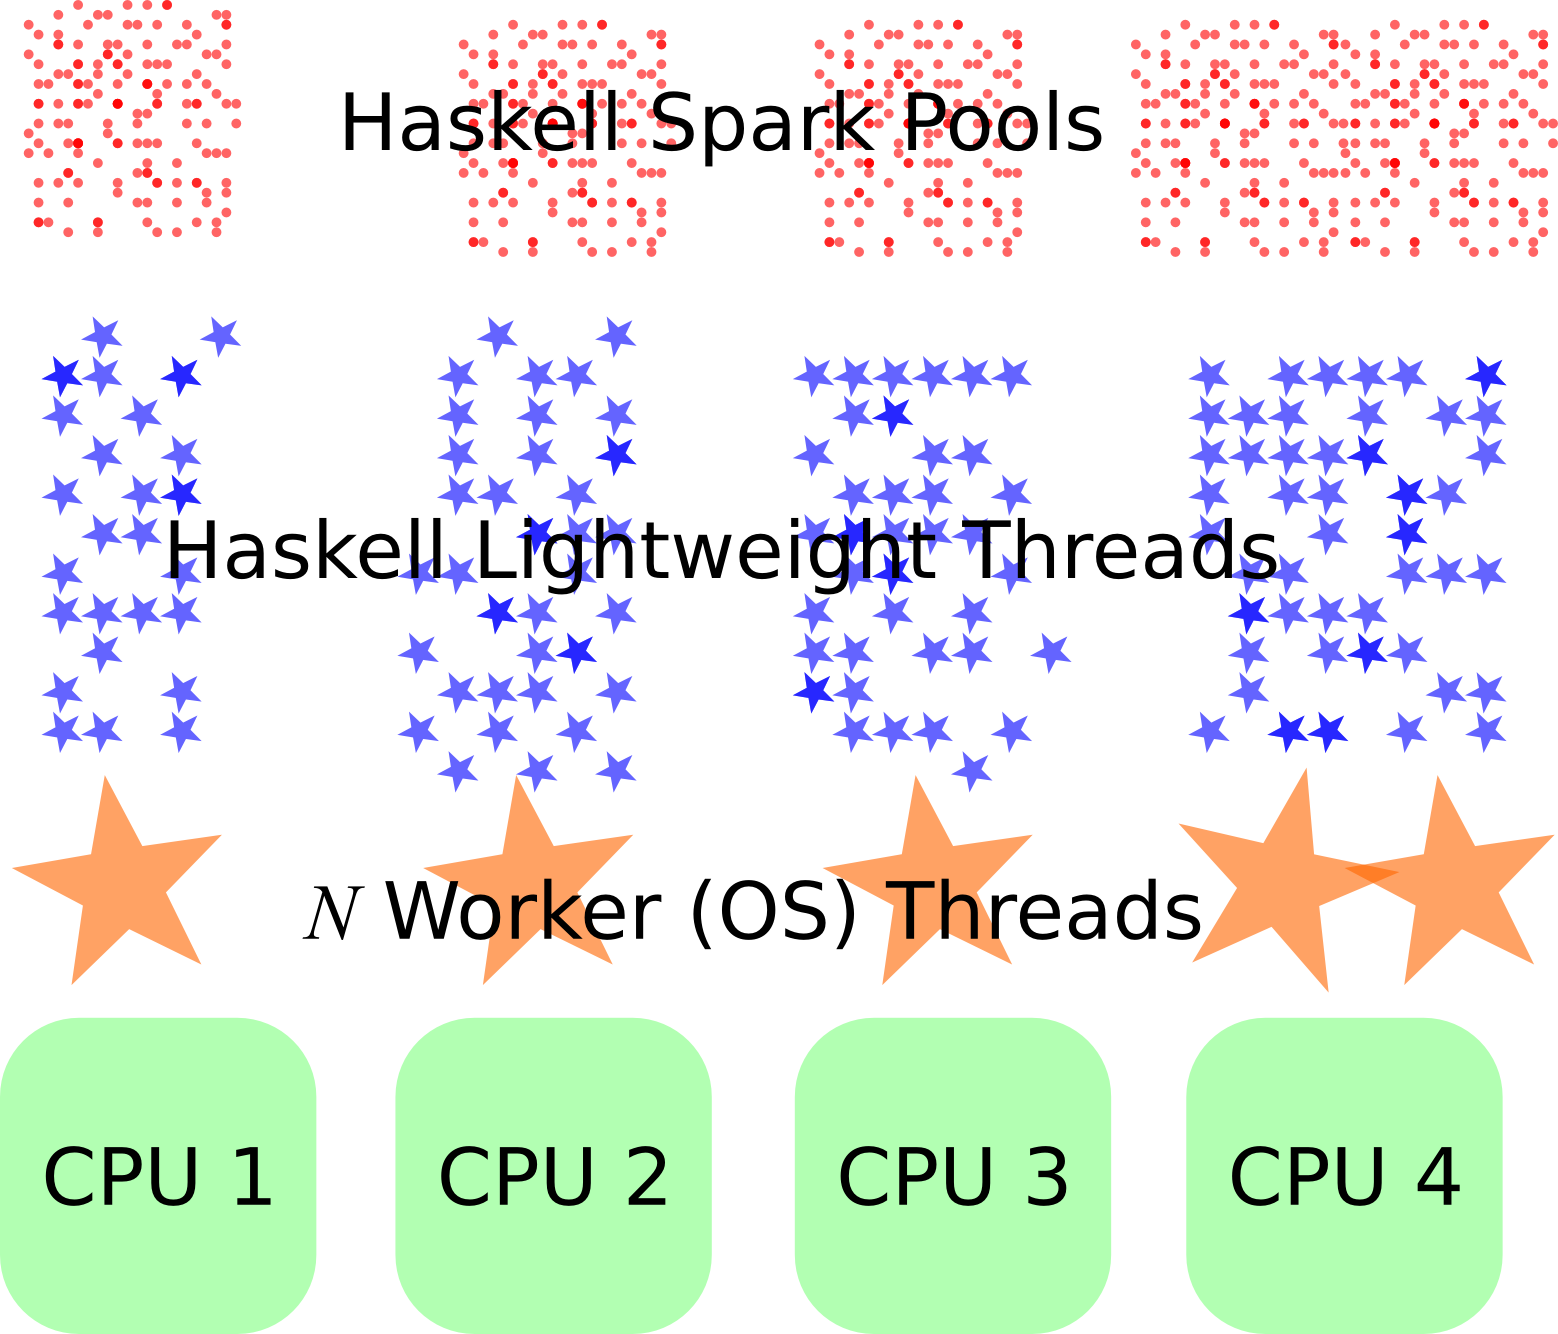
\includegraphics[width=0.6\textwidth, keepaspectratio]{imgs/haskell-threads.png}
\caption{Visualised difference between Haskell threads and spark pools and how they are mapped to OS threads.}
\end{figure}
\noindent
Haskell threads are created from sparks automatically as needed by the runtime system. A thread has a \textbf{Thread State Object} (TSO) that contains the following:
\begin{itemize}
\item A private stack
\item Private registers
\item A pointer to the spark that created the thread
\item Stats (BLOCKED, RUNNING etc.)
\item Other information needed to run the thread
\end{itemize}
All threads share a common heap for dynamic memory. 

\end{document}